\documentclass[reqno,12pt,oneside]{report} % right-side equation numbering, 12 point font, print one-sided
%\documentclass[reqno,12pt,twoside,openright]{report} % right-side equation numbering, 12 point font, print two-sided, Chapters start on odd pages. Rackham only accepts one-sided, so this is for personal printings.

\usepackage{rac}         % Use Rackham thesis style file
%\usepackage{aas_macros}  % To allow the reading of ADS journal references in the bibliography
\usepackage[intlimits]{amsmath} % Puts the limits of integrals on top and bottom
\usepackage{amsxtra}     % Use various AMS packages

\usepackage{amsthm}
\usepackage{amssymb}
\usepackage{graphicx}    % Add some packages for figures. Read epslatex.pdf on ctan.tug.org

\usepackage{rotating}
\usepackage{color}
\usepackage{xspace}
\usepackage{mdframed}
\usepackage{epsfig}
\usepackage{subfigure}   % To make subfigures. Read subfigure.pdf on ctan.tug.org
\usepackage{multirow}

\usepackage{verbatim}
\usepackage[numbers]{natbib}      % Allows you to use BibTeX
\usepackage{acronym} % For the List of Abbreviations. Read acronym.pdf on ctan.tug.org
\usepackage{booktabs}% http://ctan.org/pkg/booktabs
\newcommand{\tabitem}{~~\llap{\textbullet}~~}
\usepackage{indentfirst}
\usepackage{enumitem}
\usepackage{setspace}
\usepackage[T1]{fontenc}
\usepackage[utf8]{inputenc}
%\usepackage[options ]{algorithm2e}
\usepackage{algpseudocode}
\usepackage{ifthen}
%\usepackage{mathptmx} 
%\usepackage[acronym]{glossaries}
%\usepackage{nomencl}
%\usepackage[noend]{algpseudocode}
%\usepackage[linesnumbered,ruled,vlined]{algorithm2e}

\usepackage[intoc]{nomencl}
\usepackage{tikz}
\usetikzlibrary{shapes.geometric, arrows}

\usepackage{url}
%\usepackage{breakurl}
%\usepackage[breaklinks]{hyperref}
% \usepackage{hyperref}
 
 \usepackage{algorithm,algpseudocode}


%\usepackage[latin1]{inputenc}
%\usetikzlibrary{shapes,arrows}
\tikzstyle{startstop} = [rectangle, rounded corners, minimum width=3cm, minimum height=1cm,text centered, draw=black, fill=red!30]
\tikzstyle{io} = [trapezium, trapezium left angle=70, trapezium right angle=110, minimum width=3cm, minimum height=1cm, text centered, draw=black, fill=blue!30]
\tikzstyle{process} = [rectangle, minimum width=3cm, minimum height=1cm, text centered, draw=black, fill=orange!30]
\tikzstyle{decision} = [diamond, minimum width=3cm, minimum height=1cm, text centered, draw=black, fill=green!30]
\tikzstyle{arrow} = [thick,->,>=stealth]

%%%<


\usepackage[nottoc,notlof,notlot]{tocbibind}
\renewcommand\bibname{References}

\makenomenclature
%\makenomenclature
  % Allows you to specify the line spacing
%\doublespacing
\onehalfspacing %for 1.5 spacing, %\doublespacing for 2.0 spacing.
\newcommand{\sun}{\ensuremath{\odot}} % sun symbol is \sun
%%%%%%%%%%%%%%%%%%%%%%%%%%%%%%%%%%%%%%%%%%%%%%%%%%%%%%%%%%%%%%%%%%%%%%%%%%%%%%%

% Various theorem environments. All of the following have the same numbering
% system as theorem.

\theoremstyle{plain}
\newtheorem{theorem}{Theorem}
\newtheorem{prop}[theorem]{Proposition}
\newtheorem{corollary}[theorem]{Corollary}
\newtheorem{lemma}[theorem]{Lemma}
\newtheorem{question}[theorem]{Question}
\newtheorem{conjecture}[theorem]{Conjecture}
\newtheorem{assumption}[theorem]{Assumption}

\theoremstyle{definition}
\newtheorem{definition}[theorem]{Definition}
\newtheorem{notation}[theorem]{Notation}
\newtheorem{condition}[theorem]{Condition}
\newtheorem{example}[theorem]{Example}
\newtheorem{introduction}[theorem]{Introduction}

\theoremstyle{remark}
\newtheorem{remark}[theorem]{Remark}
%%%%%%%%%%%%%%%%%%%%%%%%%%%%%%%%%%%%%%%%%%%%%%%%%%%%%%%%%%%%%%%%%%%%%%%%%%%%%%%

\numberwithin{theorem}{chapter}     % Numbers theorems "x.y" where x
                                    % is the section number, y is the
                                    % theorem number

%\renewcommand{\thetheorem}{\arabic{chapter}.\arabic{theorem}}

%\makeatletter                      % This sequence of commands will
%\let\c@equation\c@theorem          % incorporate equation numbering
%\makeatother                       % into the theorem numbering scheme

%\renewcommand{\theenumi}{(\roman{enumi})}

%%%%%%%%%%%%%%%%%%%%%%%%%%%%%%%%%%%%%%%%%%%%%%%%%%%%%%%%%%%%%%%%%%%%%%%%%%%%%%

% If printing two-sided, this makes sure that any blank page at the
% end of a chapter will not have a page number.
\makeatletter
\def\cleardoublepage{\clearpage\if@twoside \ifodd\c@page\else
\hbox{}
\thispagestyle{empty}
\newpage
\if@twocolumn\hbox{}\newpage\fi\fi\fi}
\makeatother

%%%%%%%%%%%%%%%%%%%%%%%%%%%%%%%%%%%%%%%%%%%%%%%%%%%%%%%%%%%%%%%%%%%%%%%%%%%%%%

%This command creates a box marked ``To Do'' around text.
%To use type \todo{  insert text here  }.

\newcommand{\todo}[1]{\vspace{5 mm}\par \noindent
\marginpar{\textsc{To Do}}
\framebox{\begin{minipage}[c]{0.95 \textwidth}
\tt\begin{center} #1 \end{center}\end{minipage}}\vspace{5 mm}\par}



\begin{document}
%\bibliographystyle{ieeetr}
%\bibliographystyle{plain}    % Set the bibliography style. agu04, plain, alpha, etc.
% Title page as required by Rackham dissertation guidelines
\titlepage{A Convolutional Neural Network Based Human Expression Analysis using Jahangirnagar University dataset}{ 152395}{Professional Masters in Information Technology}
{Information Technology}{December 2020}
{Dr. M Shamim Kaiser, Professor}

% Begin the front matter as required by Rackham dissertation guidelines
\initializefrontsections

% Optional Frontispiece
%\frontispiece{\includegraphics[width=6in]{Intro/Happy} Find a cool picture to go here.}

% Optional, but recommended, Copyright page
%\copyrightpage{Your Name}

% Page numbering. If you don't include a frontispiece or copyright page, you'll need to change this for two-sided printing.
\makeatletter
\if@twoside \setcounter{page}{4} \else \setcounter{page}{1} \fi
\makeatother

% Optional Dedication page
%\dedicationpage{To Our Beloved Parents}


%Optional declaration page
\startdeclarationpage
I hereby declare that this thesis is based on the results found by ourselves. Materials
of work found by other researcher are mentioned by reference. This thesis, neither in
whole nor in part, has been previously submitted for any degree.

\vspace{1in}


\noindent   \rule{3.5cm}{1pt} \\
   Roll:152395 \\


\label{declaration}


%Optional Certificate page
\startcertificatepage
The project titled “Thesis Title” submitted by Student-Name, ID: xxxx, Session: xxx, has been accepted as satisfactory in partial fulfillment of the requirement for the degree of Professional Masters in Information Technology on the 3rd of January 2023.

%\bigskip

\bigskip
\bigskip
\bigskip

\noindent \begin{tabular}{l}

  % after \\: \hline or \cline{col1-col2} \cline{col3-col4} ...
  \rule{4cm}{1pt} \\
  Dr. M. Shamim Kaiser\\ % replace it
  Supervisor\\

\end{tabular}


%Accepted and approved in partial fulfilment of the requirement for the degree Professional Master in Information Technology.


\begin{center}
   \textbf{BOARD OF EXAMINERS}
\end{center}
\noindent \begin{tabular}{lp{1cm}r}
\centering
  % after \\: \hline or \cline{col1-col2} \cline{col3-col4} ...
  \rule{4cm}{1pt}&\\
     Dr. Mohammad Abu Yousuf  &&Coordinator  \\
     Professor, IIT, JU  & & PMIT Coordination Committee  \\
     & &  \\
     \rule{4cm}{1pt}&\\
    Dr. M. Shamim Kaiser  & &Member, PMIT Coordination Committee   \\
     Professor, IIT, JU  & &\& Director, IIT\\
    & &  \\
     \rule{4cm}{1pt}&\\
     Dr. Shamim Al Mamun & &Member  \\
      Associate Professor, IIT, JU  & &PMIT Coordination Committee  \\
     &  \\
     \rule{4cm}{1pt}&\\
     Dr. Mohammad Shahidul Islam   & &Member  \\
      Associate Professor, IIT, JU  & &PMIT Coordination Committee  \\
      &  \\
     \rule{4cm}{1pt}&\\
     Dr. Md. Sazzadur Rahman  & &Member  \\
      Associate Professor, IIT, JU  & &PMIT Coordination Committee  \\
     
  %\rule{4cm}{1pt} & \rule{4cm}{1pt} & \rule{4cm}{1pt}\\
   

\end{tabular}


%\noindent \begin{tabular}{p{5cm}p{4cm}p{5cm}}
%\centering
  % after \\: \hline or \cline{col1-col2} %\cline{col3-col4} ...
   %  &  &   \\
    % &  &   \\
     %&  &   \\
  %\rule{4cm}{1pt} &  & \rule{3.5cm}{1pt}\\
  %Jesmin Akhter &   &K M Akkas Ali\\
  %Chairman &   &Member\\
   %  &  &   \\
    % &  &   \\
  %\rule{3.5cm}{1pt}& & \rule{3.5cm}{1pt}\\
   %Shamim Al Mamun&   &Prof. Dr. M. A. Mottalib \\
  %Member &   &Member (External) \\
%\end{tabular}


\label{Certificate}



% Optional Acknowledgements page
\startacknowledgementspage
We feel pleased to have the opportunity of expressing our heartfelt thanks and gratitude to those who all rendered their cooperation in making this report.








This thesis is performed under the supervision of Dr. M. Shamim Kaiser, Associate professor, Institute of Information Technology (IIT), Jahangirnagar University, Savar, Dhaka. During the work, he has supplied us a number of books, journals, and materials related to the present investigation. Without his help, kind support and generous time spans he has given, we could not perform the project work successfully in due time. First and foremost, we wish to acknowledge our profound and sincere gratitude to him for his guidance, valuable suggestions, encouragement and cordial cooperation.

We express our utmost gratitude to Dr. M Mesbahuddin Sarker, Director, IIT, Jahangirnagar University, Savar, Dhaka, for his valuable advice that have encouraged us to complete the work within the time frame. Moreover, we would also like to
thank the other faculty members of IIT who have helped us directly or indirectly by providing their valuable support in completing this work.

We express our gratitude to all other sources from where we have found help. We are indebted to those who have helped us directly or indirectly in completing this work.

Last but not least, we would like to thank all the staff of IIT, Jahangirnagar University and our friends who have helped us by giving their encouragement and cooperation throughout the work.
\label{Acknowledgements}

%Optional Abstract page
\startabstractpage
Write the abstract of the project here. 






\vspace{8pt}
\textbf{Keywords:} Keyword 1, Keyword 2, Keyword 3, Keyword 4 and Keyword 5. 

\label{Abstract}




% List of Abbreviation

\listofabbreviations % Optional. Abbreviations should be stored in a file named abbr.tex
% Optional in-dissertation Abstract Page
%\startabstractpage
%{The Title of Your Dissertation}{Your Name}{Chair: Albert Einstein}
%Write the abstract of the project here. 






\vspace{8pt}
\textbf{Keywords:} Keyword 1, Keyword 2, Keyword 3, Keyword 4 and Keyword 5. 

%\label{Abstract}

\section*{
\begin{center}
  LIST OF ABBREVIATIONS
\end{center}
}

\begin{tabular}{p{2.5cm}p{10cm}}
%\textbf{\symbab}  & \symbac\\
\textbf{IIT}  & Institute of Information Technology\\
\textbf{JU}  & Jahangirnagar University \\
\textbf{IIT}  & Institute of Information Technology \\
\textbf{IIT}  & Institute of Information Technology \\ 
% double back slash refers to newline
\textbf{QoS}  & Quality of Service \\

\end{tabular}



% List of Notatoin
\listofnotations
\section*{
\begin{center}
 LIST OF NOTATIONS
\end{center}
}


\begin{tabular}{p{2.5cm}p{10cm}}
%\textbf{\symbab}  & \symbac\\
$\alpha$  & Define alpha\\
$\max$  & maximum\\
$\cos{\theta}$ & maximum\\
$x$ & maximum\\ % for equation mode use $$; & next column

\end{tabular}

%\input{Preface}
%\label{Preface}
% Table of contents, list of figures, etc.
\listoffigures   % Required if there is more than one figure
\listoftables        % Required if there is more than one table
\tableofcontents     % Required

%\startprefacepage
\printnomenclature[1.5cm]

%%%%%%%%%%%%%%%%%%%\printnomenclature
%\clearpage



%\renewcommand{\arraystretch}{1.70}
%\begin{tabular}{p{2.5cm}p{10cm}}
%\centering
  %\rule{3.5cm}{1pt} & \rule{3.5cm}{1pt} & \rule{3.5cm}{1pt}\\
%  $\alpha$ & Define Alpha\\
%$\symba $ & \symbb\\
%$\symbc $ & \symbd\\
%$\symbe $ & \symbf\\
%$\symbg $ & \symbh\\
%$\symbi $ & \symbj\\
%$\symbk $ & \symbl\\
%$\symbm $ & \symbn\\
%$\symbo $ & \symbp\\
%$\symbq $ & \symbr\\
%$\symbs $ & \symbt\\
%$\symbu $ & \symbv\\
%$\symbw $ & \symbx\\
%\end{tabular}
%\newpage
%\begin{tabular}{p{2.5cm}p{10cm}}









%\listofmaps          % Required if there is more than one map
%\listofappendices    % Required if there is more than one appendix
%%%%--------------------------------------------------------------------------------
\startthechapters
% The individual files for each of the chapters are put here.
% Save each chapter of your thesis to a seperate tex file
% and then use the \input command to include this file in your
% thesis.  For instance you can save a file to "intro.tex" and
% then type \input{intro}.

 %\chapter{Introduction}
 \label{chap:Intro}
 

\chapter{Introduction}

%\label{chap:GettingStarted}
\section{Overview}
This section includes the overview of the report. 

\section{Motivation}

\subsection{Image Processing}






\section{Problem Statement}
This section includes problem statement

\section{Motivation}
Analyzing research interest and existing work in the field of IoT, security is the most vital issue that drives the researcher towards the field. As architecture and application is going large day by day, security has become the important challenge for IoT. Interest in this field is proportionally increases with the Heterogeneity of this network. 

\begin{figure}
    \centering
    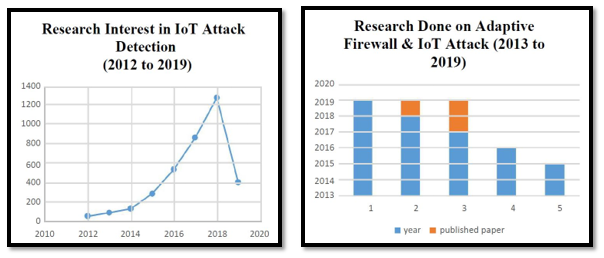
\includegraphics[scale=0.5]{Chap1/motivation.PNG}
    \caption{Research Interest in Field of IoT}
    \label{fig:motivation}
\end{figure}

 In figure \ref{fig:motivation} shows the existing research interest in IoT Attack Detection which is increasing day by day for last few years whereas for detecting attack concept of Adaptive Firewall is not so common and used term in this field. This drives us motivated to design adaptive firewall for attack detection and to block illegitimate traffic on IoT Network Model.
\section{Objective}
%The Overview goes here \cite{r1}.
IoT network model and devices are vulnerable to different kind of attacks. These attacks may vary to different category, so have different approach to detect and block them. The goal of this research is to study and identify potential IoT security attacks, detect and mitigate them by using Adaptive firewall concept. Additionally, machine learning should be considered for classifying attacks and identifying attacks \cite{c4}.
Specific goals of this thesis that should be mentioned:

\begin{itemize}
    \item Analyze network traffic to detect the malicious ones that tries to hamper the network.
    \item Find the characteristics of perception layer’s attack to identify specific attacks.
    \item Extract features from the generated traffic datasets to train machine learning classifiers and apply them to recognize attacks.Propose a centralized attack detection model.
    \item Design a rule based and ANN based FIS to help SDN controller to evaluate specific attack probability and block the suspicious ones.
    \item Maintaining the performance of the network.
\end{itemize}

This proposed model also answers the following questions:
\begin{enumerate}
    \item What are the major challenges that have guided security in IoT?
    \item What is the best attack detection way for IoT network model?
    \item Is there any generalized approach for detecting different layer attack?
    \item What is the best way to detect a single layer attack?
\end{enumerate}

\section{Assumptions \& Limitations}
Though a centralized and efficient model has been proposed to detect attacks on IoT network, it has limitations on which further studies should be done:
\begin{itemize}
    \item No approach has been mentioned for network and application layer security.
    \item No real time data has been used for the traffic analysis.
    \item Here feature Extraction and Selection method has been analyzed but no implementation has been shown.
    \item No comparison among different IDS model has been analyzed so can’t be declared it as the optimal way. 
    \item No performance measure of used Classifier is evaluated here.
\end{itemize}

\section{Research Outline}
Rest of the report is structured as follows: In \textbf{Chapter \ref{chap:2}} a literature study on related work is given including explanations for the most important terms used in this thesis-basic concept and architecture of IoT Network Model, Attacks on IoT, Concept and architecture of SDN, different model of IDS, Concept of Firewall has been discussed through this chapter. \textbf{Chapter III}  introduces system model including system architecture, algorithm and flowchart of working procedure of entire system model. \textbf{Chapter IV} explains the details of traffic analysis techniques, Feature Extraction and Selection mechanism and tools for this mechanism and reasoning how these mechanisms work for our model. \textbf{Chapter V} discusses about the simulation and model performance, to analysis result of the model it describes the basic mechanism of attack detection like Fuzzification, NSL KDD dataset, FIS, Defuzzification,Simulation and confusion matrix. Lastly in \textbf{Chapter VI} future work and conclusion is mentioned. 

\section{Limitation}
Bla bla bla
\label{sec:EffSearch} 
\index{Search engines!using effectively} %index will be created
%The rest of this report is organized as follows.






% \chapter{Literature Survey}
 
\chapter{Literature Review}
\label{chap:2}

\section{Related Work}

\subsection{Soft Engg}

 Several studies investigated diabetes data and constructed models to predict diabetes. Equation \ref{eq:1} give

\begin{equation} \label{eq:1}
    y=\sum_i x_i+C^2+\frac{1}{\cos{\theta}}
\end{equation}

Figure \ref{tab:sub} shows bla bla
\begin{table}[ht!]
    \centering
     \caption{Supervised Machine Learning Classifier}
     \vspace{2pt}
    \begin{tabular}{lrp{3in}}
    \hline
        \textbf{hello} & \textit{JU} & Header 2  \\ \hline
         Shamim & KMA & In this step, we will describe some supervised machine learning classifiers namedLogistic Regression, k-nearest neighbors, Support Vector Machine, Decision Tree,Gaussian Naive Bayes, Random Forest, Gradient Boosting and Linear DiscriminantAnalysis. \\  \hline
    \end{tabular}
    \label{tab:sub}
\end{table}

\section{ Machine Learning Types}

\section{Supervised Machine Learning Classifiers}

In this step, we will describe some supervised machine learning classifiers named Logistic Regression, k-nearest neighbors, Support Vector Machine, Decision Tree, Gaussian Naive Bayes, Random Forest, Gradient Boosting and Linear Discriminant Analysis. 

\subsection{Logistic Regression (LR)}

Logistic Regression (LR) is a supervised machine learning data classification algorithm that mines real-valued features from the input, multiplies each of them by a weight, adds them, and transfers the sum through a sigmoid function to produce a probability. A threshold is used to finalize a decision \cite{DSR}. A solution for classification of our data set is LR which Instead of fitting a straight line or hyperplane uses the logistic function to squeeze the output of a linear equation between 0 and 1. The logistic function is defined as:

\[Logistic (\eta) = 1/(1 + exp (-\eta))\]

As $\eta$ goes from $-\infty$ to $\infty$, logistic ($\eta$) goes from 0 to 1, a “squashing function”. In our study, we used a maximum 4000 iterations to converge the output.


\subsection{k-nearest neighbors (KNN) }
 (KNN) is a non-parametric process we used for diabetic data classification. In KNN a data is classified by a majority vote of its neighbors, with the data being allotted to the class most mutual amongst its K nearest neighbors estimated by a distance function. If K = 1, then the data is simply allotted to the class of its nearest neighbor. KNN algorithm is as below : 

\begin{algorithm}
\caption{KNN}
\label{pseudoPSO}
\begin{algorithmic}[1]
\State Let $m$ be the number of training data samples. Let $p$ be an unknown point that needs to be classified
\State Storing the training samples in an array of data points $arr[]$. Each element of this array denotes a tuple $(x, y)$.

\For{$i=0$ to $m$}
    \State Calculating distance $d(arr[i], p)$
   
\EndFor
\State Making set $S$ of $K$ smallest distances achieved. Each of these distances resembles an already classified data point
\State Returning the majority label among $S$
\end{algorithmic}
\end{algorithm}


\subsection{Decision Tree (DT)}
A DT is a classifier that recursively performs partition of the instance space. The decision tree contains nodes that form a tree, a node called “root” that has no incoming edges is the starting point of the tree. All other nodes have one incoming edge. The leaf nodes are known as decision nodes. The child node is nominated by computing Information Gain (IG).

Information Gain = Entropy(parent) - [weights average] * Entropy(children)

Entropy($Ci$) = -P($xi$) log P($xi$), where P($xi$) is the probability of child node $i$. 

Node with the highest IG will be the parent for next level. This process is continued until it gets a leaf node and completed decision tree. 

The algorithm for generating a decision tree is as below :

\begin{algorithm}
\caption{DT}
\label{pseudoPSO1}
\begin{algorithmic}[1]

\State  Create (T) 
\State Calculate frequencies (Ci, T)
\State  If all instances belong to the same class, returning leaf 
\State for every attribute a test is set for splitting criteria. An attribute that satisfies the test is test node K
\State  Repeating Create (Ti) on each partition Ti.Adding those nodes as children of node K

\end{algorithmic}
\end{algorithm}





\subsection{Gaussian Naive Bayes (GNB)}
The GNB classifier is a probability distribution function having the effect of associating neural activation to the means and variances of activation in various impulse conditions. The production of the classifier is a condition-label.  The classifier creates hypothesis that the classes have Gaussian normal distributions.

The z-score distance between the inputted point and each class-mean is estimated for each data point, namely the distance from the class mean divided by the standard deviation of that class.

\begin{equation*}
    Z_A=\frac{(x-\mu_A)}{\sigma_A}
\end{equation*}

According to the equation for a Gaussian normal distribution, each z-score is then converted into a probability value which is used for observing data point x. The co-variance between dimensions is not modelled by GNB classifier.


\subsection{Random Forest (RF)}
RF is a collective algorithm which was modelled from trees algorithm and Bagging algorithm. It works fine with a data set with a large number of input variables. It is a meta estimator that creates a number of decision tree classifiers on different sub-samples of the data set and uses mean value to increase the accuracy of the model and control over-fitting. Suppose training data set is given as: [X1, X2, X3, X4] with labels as [L1, L2, L3, L4] respectively, random forest algorithm may create three decision trees taking input of subset for example, [X1, X3, X4], [X2, X3, X4] and [X1, X2, X4]. Finally, it predicts class based on the majority of votes from each of the decision trees generated. Generally, the more trees in the forest the more robust and reliable the forest is. The random forest classifier works in the same way, the higher the number of trees in the forest gives higher accuracy output .


\subsection{Gradient boosting (GB)}
GB includes three components: a loss function that is to be optimized, a weak learner that makes predictions and an additive model which will add weak learners to minimize the loss function. 









\section{Research Gap}
Analyzing related works in this field an be noticed some shortcoming in the security measurements of IoT network. \textbf{Firstly}, there is no centralized detection method is mentioned, every layer has specific detection way method but as IoT is becoming a heterogenous network a centralized model should be proposed in controller which will control the traffic of every subpart of network. \textbf{Secondly}, by using KDD Dataset most commonly \textbf{DDoS, Probe, U2R, R2L} attack has been detected but with advancing technology intruder can attack the network in many other ways. \textbf{Thirdly}, no time efficient optimal way is mentioned to detect attack. \textbf{Fourthly}, traditional firewall can’t detect any encrypted incoming packet which can be removed by using adaptive firewall concept but still much work has not done yet regarding this problem \cite{mahmud_brain-inspired_2018,8742551,noauthor_coronavirus_nodate}.

\begin{figure}[!htb]
    \centering
    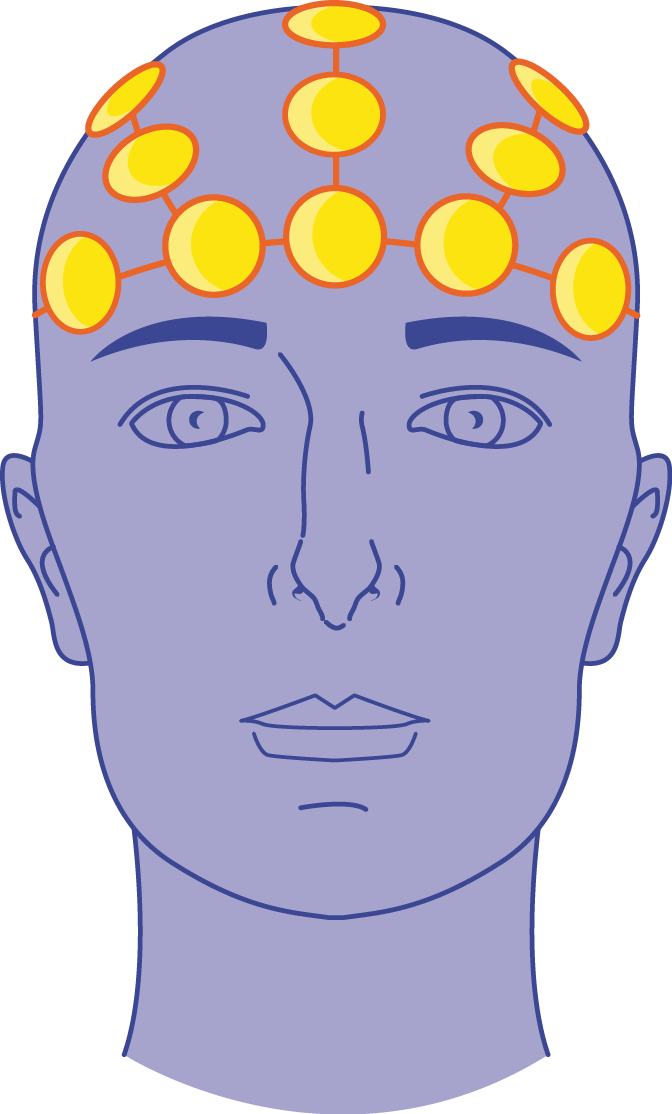
\includegraphics[scale=0.5]{Chap2/EEGonbrain.png}
    \caption{EEG probe on brain}
    \label{fig:my_label}
\end{figure}


%\chapter{System Model}
 \chapter{System Model}
\section{Proposed Architecture}


As our main purpose is to secure the network from different types of attacks which are mostly related with the traffic, we have come up an idea to integrate SDN with IoT for better performance, security and access control mechanism.

\begin{figure}[ht]
   \centering
   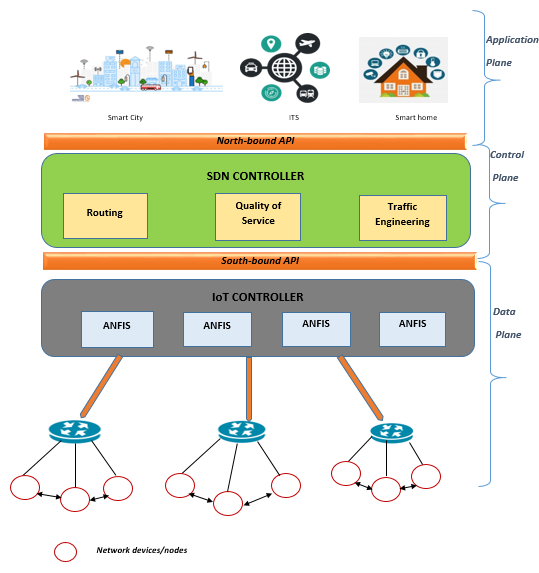
\includegraphics[width=5.5in]{Chap3/proposedmodel.png}
   \caption{System Model}
   \label{fig:model}
\end{figure}








%\chapter{Simulation Results and Discussion}
\chapter{Algorithm Analysis}

\section{Traffic Analysis}



A SDN based IoT infrastructure basically provides free-flow of data from sensors and wireless devices and the efficiency of the network depends on the management and security of traffic. Network traffics are dynamic and hence its more prone to malicious attacks such as DDOS, MITM, Replay, Side Channel etc.

\subsection{Traffic Analysis Technique}

There are various classification techniques to classify the network traffic, but among these the following three techniques are mostly used-port based, payload/DPI (Deep Packet Inspection) based and ML (Machine Learning)-technique.

In \textbf{Port-based technique}, IP addresses are identified and used to classify the corresponding applications which are registered under Assigned Number Authority (AINA). In the other side, \textbf{Payload-based} or \textbf{Deep Packet Inspection(DPI)} are basically used to classify dynamic port numbers (peer to peer applications) and packets are analyzed for signatures and authentications of network applications of traffic.\textbf{ ML (Machine Learning)-technique} uses trained classifiers as input for traffic classification based on the data set.

For our proposed system, to analysis the traffic efficiently we are applying ML-technique, as port-based classification doesn’t provide the identification of dynamic ports and payload-based doesn’t work for encrypted traffic and requires continuous updating of signature patterns of new applications. ML-technique overcomes these shortcomings of the following classification techniques and works more efficiently to classify data packets \cite{6091325,Santi-journal}.


\begin{figure}[ht]
    \centering
    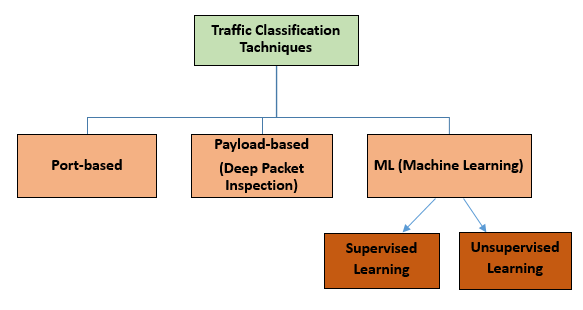
\includegraphics{Chap4/trafficanalysis.png}
    \caption{Traffic Analysis Technique}
    \label{fig:traffic_analysis}
\end{figure}

\textbf{ML (Machine Learning)- Technique}

Machine learning is used for dynamic analysis for traffic and uses \textbf{WEKA} tool for detection method. It has two techniques for classification- supervised and unsupervised. In \textbf{Supervised} technique there is a training data set as input to train the system model for the expected output but in \textbf{unsupervised} technique there is no training/known data set and it works based on the prior knowledge or the statistical information.



\section{Feature Extraction}

By analyzing the network traffic, we get a data set which is the combination of the malware and benign data packets and this is the first major component for any malware detection system. A feature extractor is used to extract the features from the specified data set and we need to extract a group of features to detect attacks, which is not possible by extracting any specific or single feature.

\subsection{Feature Extraction Tool}
Here we are using the \textbf{Wireshark} and \textbf{Net Mate tool} for the corresponding live data packet capturing and feature extraction purpose.
\begin{enumerate}
    \item \textbf{Wireshark:} Wireshark is an open source software and an efficient network packet analyzer. Wireshark captures the network traffic from various wireless devices and displays them with very detailed protocol information and save the captured data packet. It can also export some or all packets in a number of capture file formats and filter them on many criteria. The basic features of Wireshark tools are-
    \begin{itemize}
        \item Capture traffics from live network or read data from already captured file.
        \item Terminal version, named Tshark or GUI is used to browse captured traffic.
        \item Display filter is used to refine and edit traffic programmatically.
        \item For dissecting protocols, Plug-ins is developed.
        \item Captured traffic can be used to detect VoIP calls when compatible encoding is used for encoding. 
        \item Only selected traffic appears with several timers, settings and filters.
    \end{itemize}
    \item \textbf{Net Mate Tool:} After capturing data packets, the features are extracted using Net Mate tool as features depict the behavioral description of traffic. Net Mate includes two types of modules:
    \begin{itemize}
        \item Packet Processing Modules designed to implement different metrics 
        \item Export Module that implement different output module
    \end{itemize}
    Our concerned flow features are implemented in \textbf{Packet Processing Module}. Two different types of rules are used to produce the output: description rules and recognition rules.
\end{enumerate}
\begin{figure}[ht]
    \centering
    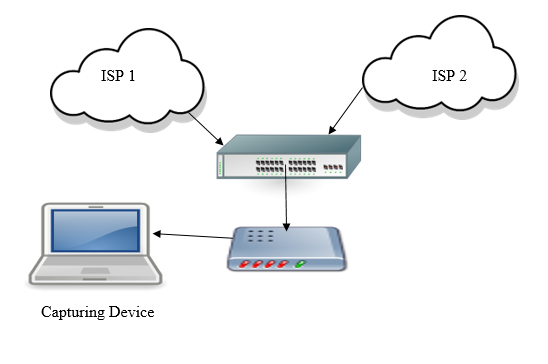
\includegraphics[width=5in]{Chap4/FeatureExtraction.PNG}
    \caption{Feature Extraction Process}
    \label{fig:feature_extraction}
\end{figure}
\section{Feature Selection}

Feature Selection is an important step after traffic analysis to detect the abnormality occurring in a system. It can be defined as automatic selection of attributes in data samples that are most relevant to the predictive modeling problem. It does the mapping to excludes the irrelevant or redundant attributes and specifically defines most prominent for the better performance of the system.

As in our proposed system we are working on a large amount of a traffic of a network so feature selection should be done for the following requirements:
\begin{itemize}
    \item To create an accurate predictive model that will give a better accuracy whilst requiring less data.
    \item it reduces the complexity of a model and makes it easier to interpret the required result.
    \item It enables the model to train faster on data sample as there is no redundant attributes.
    \item This method also reduces the problem of over fitting by enhancing the generalization in the model.
\end{itemize}
\subsection{Selection Method}
There are mainly three methods that are used in feature selection:
\begin{enumerate}
    \item \textbf{Filter Method:} Here features are selected on the basis of their scores in various statistical tests for their correlation with the outcome variable which is Machine Language Independent.\textbf{Pearson’s Correlation, LDA, ANOVA, Chi- Square}  are the methods which are used to define correlation among the features.
    \item \textbf{Wrapper Method:} This method considers the selection of a set of features as a search problem or algorithm to validate the prediction where different combinations are prepared, evaluated and compared to other combinations. After evaluating it assigns a score based on model accuracy. It can always provide the best subset of features. But this method has a high computational cost.
    \item \textbf{Embedded Method:} This method tries to combine the efficiency of other two methods and performs the selection of variables in the process of training and is usually specific to given learning machines. It basically learns which features best contribute to the accuracy of the model while the model is being created. Most common algorithms are the \textbf{LASSO, Elastic Net, Ridge Regression}used in this method.
\end{enumerate}

For our model \textbf{Wrapper Method} is most applicable. As at first we have analyzed network traffic and after that we have implemented a Search process for extracting Unusual features to detect our attacks. From the complete list of Feature set we have further selected the most effective features to make our feature domain more powerful.

\subsection{Selection Tool}
The immediate step after feature extraction of any attack detection procedure is feature selection which is the final input feature set to feed into the system by using any machine learning technique. To select the desired features from the extracted features set, an efficient tool-set, WEKA is used in our attack detection process.

\textbf{WEKA:} WEKA, (Waikato Environment for Knowledge Analysis), named after a flightless New Zealand bird, supports many feature selection techniques, i.e. correlation based, information gain based, learner based etc. Weka is a set of machine learning algorithms for data mining tasks. The algorithms can be used directly on dataset or it can be called from Java code. 

Weka contains tools for data pre-processing, classification, regression, clustering, association rules, and visualization. It provides SQL access with assistance of Java Database Connectivity. Weka provides four UI:
\begin{itemize}
    \item Explorer
    \item Experimenter
    \item KnowledgeFlow
    \item Simple CLI.
\end{itemize}
Explorer is the main user interface of Weka which have following panels:
\begin{enumerate}
    \item \textbf{Preprocess:} Choosing the data file.
	\item \textbf{Classify:} Applying and experimenting with different algorithms on preprocessed data files.
	\item \textbf{Cluster:} Applying different clustering tools, which identify clusters within the data file.
	\item \textbf{Association:} Applying association rules, which identify the association within the data.
	\item \textbf{Select attributes:} Seeing the changes on the inclusion and exclusion of attributes from the experiment.
	\item \textbf{Visualize:} Seeing the possible visualization produced on the data set in a 2D format, in scatter plot and bar graph output.
\end{enumerate}
The user cannot move between the different tabs until the initial preprocessing of the data set has been completed. This procedure can also be done with component based KnowledgeFlow and from Simple CLI. Experimenter provides option to compare predictive performance of machine learning algorithms on data-sets. 

\section{Feature Specification on Proposed Model}

From extraction procedure eighteen features are collected which are grouped into nine features for the convenience of our work.And these nine features are taken as input for the further process.The mapping or selection of features are simplified as the below figure \ref{fig:feature}
\begin{figure}[ht]
    \centering
    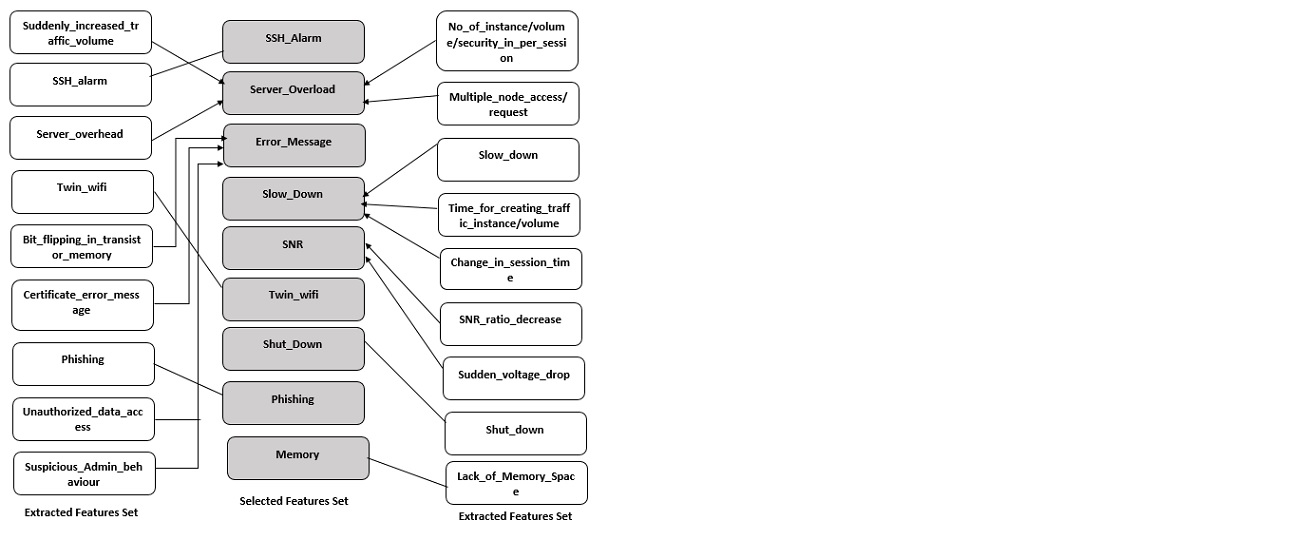
\includegraphics{Chap4/feature.jpg}
    \caption{Feature Extraction and Selection}
    \label{fig:feature}
\end{figure}

\begin{enumerate}
 \item \textbf{Server Overload:} It is one of the most common feature that happens in any kind of physical layer attack in the network. Increase of volume of data packets, excessive traffic is the indication of Server Overload. Though it’s a common feature but there is possibility of Side Channel Attack, Malicious Code and DDoS attack. 
\item \textbf{Slow Down:} It’s a common feature of DDoS and Malicious Code Attack. In DDoS there creates traffic floods in bandwidth and resources so the performance evaluation becomes very poor. It is definitely a symptom that something is wrong with the system. In malicious code there occurs illegitimate actions which creates load on the system.


\item \textbf{Sudden shut Down:} It’s the extreme case of DDoS attack in the network. a denial-of-service attack (DDoS attack) is a cyber-attack in which the perpetrator seeks to make a machine or network resource unavailable to its legitimate users by temporarily or indefinitely disrupting services of a host connected to the internet. So when network will not able to manage the overload it will just shut down.
\item \textbf{Error Message:} It is the most common characteristics of attacks that frequently occurs in IoT network model. It will generate automatically from the Operating System when it will suspect unusual activities in the network. So it is a great source of predicting that there is a third party in the network who is trying to do something illegal in the network. Features-Bit flipping in memory cells, Suspicious Admin Behavior, Unauthorized Data Access are redundant which is mapped to exclude after feature selection method. Because all these three activities are unusual and it will result an error message. DDoS, Side Channel Attack, Malicious Code Attack, Man in The Middle(MITM) attack can be suspected by this feature.
\item \textbf{	SSH Alarm:} SSH is one of the most popular communication protocols on the Internet used by admins, developers. SSH alarm is an email alert, when someone logs server via SSH (Server Secure Shell) can be pretty useful to track who is actually using server. It’s a very unique feature to track MITM attack as an intruder might not login at first attempt.
\item \textbf{Twin-WiFi:} In MITM the main aim of an intruder is to entry the network and hampers the integrity, confidentiality, authenticity of admin. To get illegal access he can adapts the method of duplicate WiFi SSID or Address that is a very prominent feature to identify that the system is being attacked by the third party.
\item \textbf{Phishing:} It’s a great threat to the security of users. It is actually a cybercrime in which targets are contacted by email, telephone or text message by someone posing as a legitimate institution to lure individuals into providing sensitive data such as personally identifiable information, banking information, credit card details, and passwords. Intruder who conducts MITM attack mostly does this to earn in an illegal way.
\item \textbf{SNR decrease:} When noise of a system increases the SNR decreases that indicates the poor performance of the system. Voltage drops with proportional to SNR, that is not definitely a good symptom for a model. It is the most prominent feature to detect the Side Channel Attack. it is caused by the information gained from the network so the noise increases which should be noticed to detect attack.
\item \textbf{Lack of Memory Space: }Malicious code is an application security threat that cannot be efficiently controlled by conventional antivirus software easily. It describes a broad category of system security terms that includes attack scripts, viruses, worms, Trojan horses, backdoors and malicious active content. So sometimes it suddenly just occupies the memory space of user device and gives warning to the user of “Memory is Full”. That’s definitely occurs a great problem of storing.

Here FIS will primarily work on these \textbf{Nine} Selected features where rules will be considered in controller to identify DDoS, MITM, Malicious Code Attack and Side Channel Attack. Rules are defined according to the priority of the features.
\end{enumerate}




%Chapter{Performance Analysis}
\chapter{Performance Analysis}
 %This section  .... table \ref{table:2} \cite{r2}
\section{Fuzzification}
\subsection{Fuzzification Method:}
\textbf{Fuzzy logic} is a form of 
\begin{itemize}
    \item Fuzzification Unit
    \item Knowledge Based Rules
    \item Decision or Controller Unit
    \item Defuzzification Unit
\end{itemize}

%% to write equation; table and figure you have to start with \begin

\begin{equation}
    y=\cos(x)+\sin(x) +\beta
\end{equation}

where $y$ is the output of the system and $x$ is the input of the system.

\begin{figure}[ht!] %H--- must here; h-- here, t--top, b--bottom
    \centering
    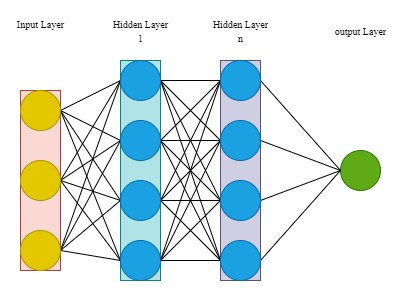
\includegraphics[scale=0.5]{Chap5/cnn1.jpg}
    \caption{CNN architecture}
    \label{fig:CNN}
\end{figure}


Figure \ref{fig:CNN} shows a CNN architecture. 


\begin{table}[]
    \centering
    \caption{Deep learning Algorithms \cite{mondal_automatic_2017}}
    \begin{tabular}{cp{2in}} %c--center, l--left, r--right; p-- width
      \hline %horizontal line
      \textbf{Name of Algorithm}   & \textbf{Description}  \\ \hline
        CNN & It includes input, hidden and output layers .\\ \hline
        RNN & It is useful for time series data. It takes output and fed into input \\ \hline
    \end{tabular}
        \label{tab:DL}
\end{table}

Table  \ref{tab:DL}     shows deep learning algorithm \cite{wiki_2016}.





%\chapter{Conclusion and Future Work}
\chapter{Conclusion and Future Work}



\section{Conclusion}
Write the conclusion 

\section{Future Work}
Write what you wanna do in future
% \label{chap:conclusion}
% \chapter{Performance Analysis}
 %This section  .... table \ref{table:2} \cite{r2}
\section{Fuzzification}
\subsection{Fuzzification Method:}
\textbf{Fuzzy logic} is a form of 
\begin{itemize}
    \item Fuzzification Unit
    \item Knowledge Based Rules
    \item Decision or Controller Unit
    \item Defuzzification Unit
\end{itemize}

%% to write equation; table and figure you have to start with \begin

\begin{equation}
    y=\cos(x)+\sin(x) +\beta
\end{equation}

where $y$ is the output of the system and $x$ is the input of the system.

\begin{figure}[ht!] %H--- must here; h-- here, t--top, b--bottom
    \centering
    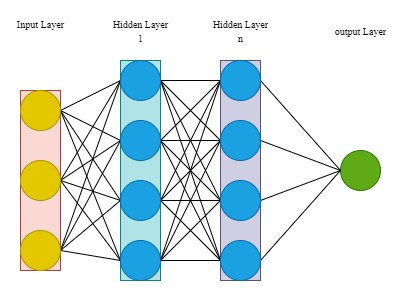
\includegraphics[scale=0.5]{Chap5/cnn1.jpg}
    \caption{CNN architecture}
    \label{fig:CNN}
\end{figure}


Figure \ref{fig:CNN} shows a CNN architecture. 


\begin{table}[]
    \centering
    \caption{Deep learning Algorithms \cite{mondal_automatic_2017}}
    \begin{tabular}{cp{2in}} %c--center, l--left, r--right; p-- width
      \hline %horizontal line
      \textbf{Name of Algorithm}   & \textbf{Description}  \\ \hline
        CNN & It includes input, hidden and output layers .\\ \hline
        RNN & It is useful for time series data. It takes output and fed into input \\ \hline
    \end{tabular}
        \label{tab:DL}
\end{table}

Table  \ref{tab:DL}     shows deep learning algorithm \cite{wiki_2016}.




%\startbibliography
 %\begin{singlespace} % Bibliography must be single spaced
%\bibliography{References}   % Use the BibTeX file ``References.bib''.
%\end{singlespace}
%%\setlinespacing{1.44}
\bibliographystyle{ieeetr}
%\bibliography{xbib}
% An external Abstract that can be printed at the end of the document,
% for separate submission to Rackham. Comment it out when not needed. - jg
%\startextabstractpage
%{The Title of Your Dissertation}{Your Name}{Chair: Albert Einstein}
%Write the abstract of the project here. 






\vspace{8pt}
\textbf{Keywords:} Keyword 1, Keyword 2, Keyword 3, Keyword 4 and Keyword 5. 

%\label{ExtAbstract}

%\bibliographystyle{alpha}
%\bibliographystyle{alpha}
\bibliography{bibfile}

\end{document}
